\begin{frame}
    \frametitle{\problemtitle}

    \begin{columns}
        \begin{column}[T]{.67\textwidth}
            \begin{itemize}
                \item Bill pours champagne into a fountain with $n \leq 3\cdot 10^5$ levels.
                \item If a bowl in some level is already filled up, then the champagne spills over to
                the first level below it with larger capacity.
                \item If the next larger level is also filled, the champagne spills over even further until eventually seeping into the ground.
                \item You are asked $q\leq 3\cdot 10^5$ queries:
                \begin{itemize}
                    \normalsize
                    \item $\text{`\texttt{+}'}$: Bill pours $x\leq 10^9$ litres of champagne into level $\ell$.
                    \item $\text{`\texttt{?}'}$: Bill wants to know how much champagne is in level $\ell$.
                \end{itemize}
            \end{itemize}
        \end{column}

        % This illustration is not 0.30 but 0.25, else the figure below does not fit.
        \illustration{0.25}{bill}{
            Bill Poucher (ICPC Executive Director, on~the~right).\\\textcopyright{} \href{https://www.huawei.com/en/news/2024/10/icpc-challenge-championship}{Huawei}, used with permission
        }
    \end{columns}

    %\vspace{1em}

    \centering
    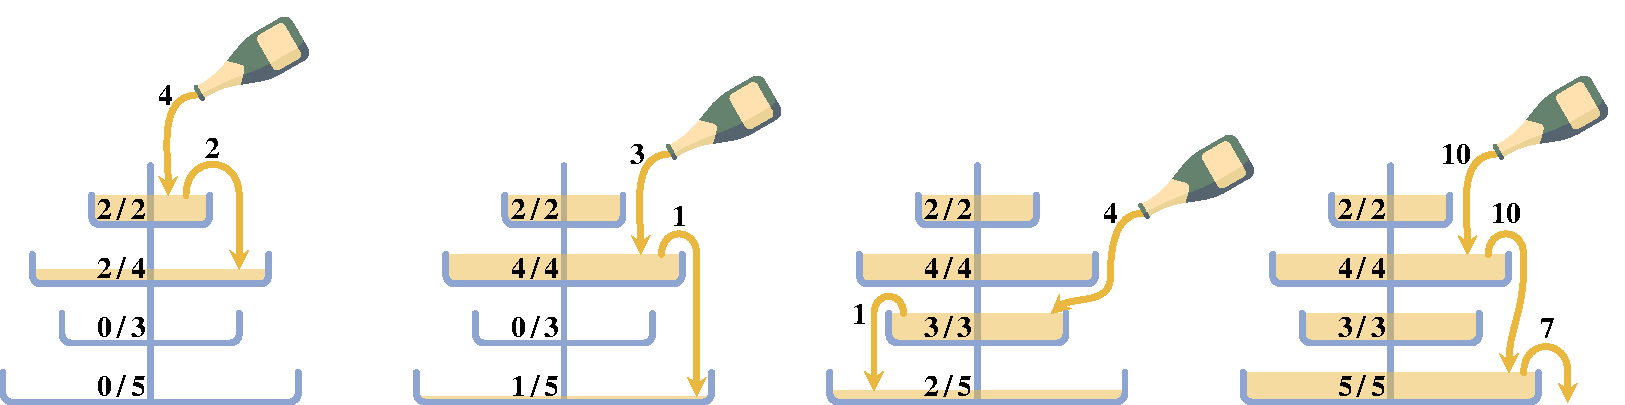
\includegraphics[width=0.7\textwidth]{sample.pdf}

    \small
    Illustration of Sample Input 2.
    The $i$th image visualizes the $i$th query of type~`\texttt{+}'.
\end{frame}
